\documentclass{article}

% Nếu compile trên Overleaf, upload kèm file neurips_2025.sty
\usepackage[preprint]{neurips_2025}

\usepackage[utf8]{inputenc}
\usepackage[T5]{fontenc}
\usepackage[vietnamese]{babel}
\usepackage{hyperref}
\usepackage{url}
\usepackage{booktabs}
\usepackage{amsmath}
\usepackage{amsfonts}
\usepackage{nicefrac}
\usepackage{microtype}
\usepackage{xcolor}
\usepackage{graphicx}
\usepackage{float}
\usepackage{array}
\usepackage{tabularx}
\usepackage{longtable}
\usepackage{multirow}
\usepackage{enumitem}
\usepackage{caption}
\usepackage{threeparttable}
\usepackage{listings}
\usepackage{setspace}


\hypersetup{
    colorlinks=true,
    linkcolor=blue!50!black,
    citecolor=blue!50!black,
    urlcolor=blue!50!black
}

\captionsetup{font=small, labelfont=bf}
\setlength{\LTleft}{0pt}
\setlength{\LTright}{0pt}
\renewcommand{\arraystretch}{1.15}

\lstset{
    basicstyle=\ttfamily\scriptsize,
    frame=single,
    breaklines=true,
    columns=fullflexible,
    keepspaces=true
}

\title{DATATHON 2026 -- Breaking Business Boundaries\\
\large}

\author{Team: Nguyễn Ngọc Hiếu \\ Nguyễn Ngọc Yến, Nguyễn Ngọc Hiếu, Huỳnh Kim Gia Bảo, Phạm Minh Trí \\ VinUniversity, Đại học Khoa học và Công nghệ Hà Nội}
\date{Tháng 4, 2026}
\begin{document}

\maketitle





% =========================================================


% =========================================================

% =========================================================
% =========================================================
\section{Trực quan hoá và phân tích dữ liệu}
\setcounter{page}{1}

\subsection{Tổng quan và cách tiếp cận}

Bộ dữ liệu gồm 3.833 ngày quan sát, từ 04/07/2012 đến 31/12/2022. Nếu tính
$\text{gross\_profit}=\text{Revenue}-\text{COGS}$, toàn giai đoạn ghi nhận khoảng
$16{,}430$ tỷ VND doanh thu, 646.945 đơn hàng và $2{,}267$ tỷ VND lợi nhuận gộp. Năm 2012 thiếu
toàn bộ các biến lượt truy cập như \texttt{sessions}, \texttt{unique\_visitors},
\texttt{page\_views} và \texttt{bounce\_rate}, nên các phân tích về lượt truy cập và tỷ lệ chuyển
đổi được giới hạn trong giai đoạn 2013--2022.

Trong giai đoạn 2013--2022, dữ liệu có 3.652 ngày, 91.452.537 phiên truy cập, 614.894 đơn hàng,
$15{,}689$ tỷ VND doanh thu và $2{,}113$ tỷ VND lợi nhuận gộp. Biên lợi nhuận gộp chung đạt
$13{,}47\%$, tỷ lệ ngày có khuyến mại đạt $46{,}7\%$. Vì khuyến mại xuất hiện khá thường xuyên,
kết quả kinh doanh cần được đọc đồng thời qua doanh thu, số đơn hàng và lợi nhuận giữ lại.

Các chỉ số chính được tính như sau:
\[
\text{conversion}=\frac{\text{order\_count}}{\text{sessions}}, \qquad
\text{AOV}=\frac{\text{Revenue}}{\text{order\_count}}, \qquad
\text{gross\_margin}=\frac{\text{Revenue}-\text{COGS}}{\text{Revenue}}.
\]
Trục phân tích chính là:
\[
\text{Revenue/day}=\text{Sessions/day}\times\text{Conversion}\times\text{AOV}.
\]
Cách tách này giúp nhìn doanh thu qua ba lớp: lượng người vào website, khả năng tạo đơn hàng và giá
trị trung bình mỗi đơn.

\subsection{Người dùng vào nhiều hơn, nhưng mua hàng ít hơn}

So với năm 2018, số phiên truy cập mỗi ngày tăng từ 25.795 lên 30.311, tương đương $+17{,}5\%$.
Tuy nhiên, tỷ lệ chuyển đổi giảm từ $0{,}74\%$ xuống $0{,}33\%$, tức giảm $55{,}9\%$. Giá trị trung
bình mỗi đơn hàng tăng từ 26.617 VND lên 32.489 VND, tương đương $+22{,}1\%$, nhưng không đủ bù
cho phần giảm chuyển đổi; doanh thu/ngày vì vậy giảm $36{,}8\%$.

Khi lấy năm 2013 làm mốc 100, đến năm 2022 số phiên truy cập/ngày đã tăng lên 162,7. Tuy nhiên,
số đơn hàng/ngày chỉ còn 46,9 và doanh thu/ngày còn 70,6. Doanh thu/ngày từng đạt đỉnh khoảng
5,75 triệu VND vào năm 2016, rồi giảm về 3,20 triệu VND vào năm 2022.

Trong khi đó, các chỉ báo tương tác gần như ổn định: số trang xem trên mỗi phiên quanh 4,31--4,40,
số phiên trên mỗi người dùng quanh 1,31--1,32, thời gian giao hàng trung bình khoảng 4,48--4,51 ngày.
Vì vậy, điểm nghẽn nhiều khả năng nằm ở bước ra quyết định mua hàng, chứ không phải ở lượng người vào
website hay mức độ tương tác ban đầu.

\begin{figure}[H]
\centering
\begin{minipage}{0.48\linewidth}
    \centering
    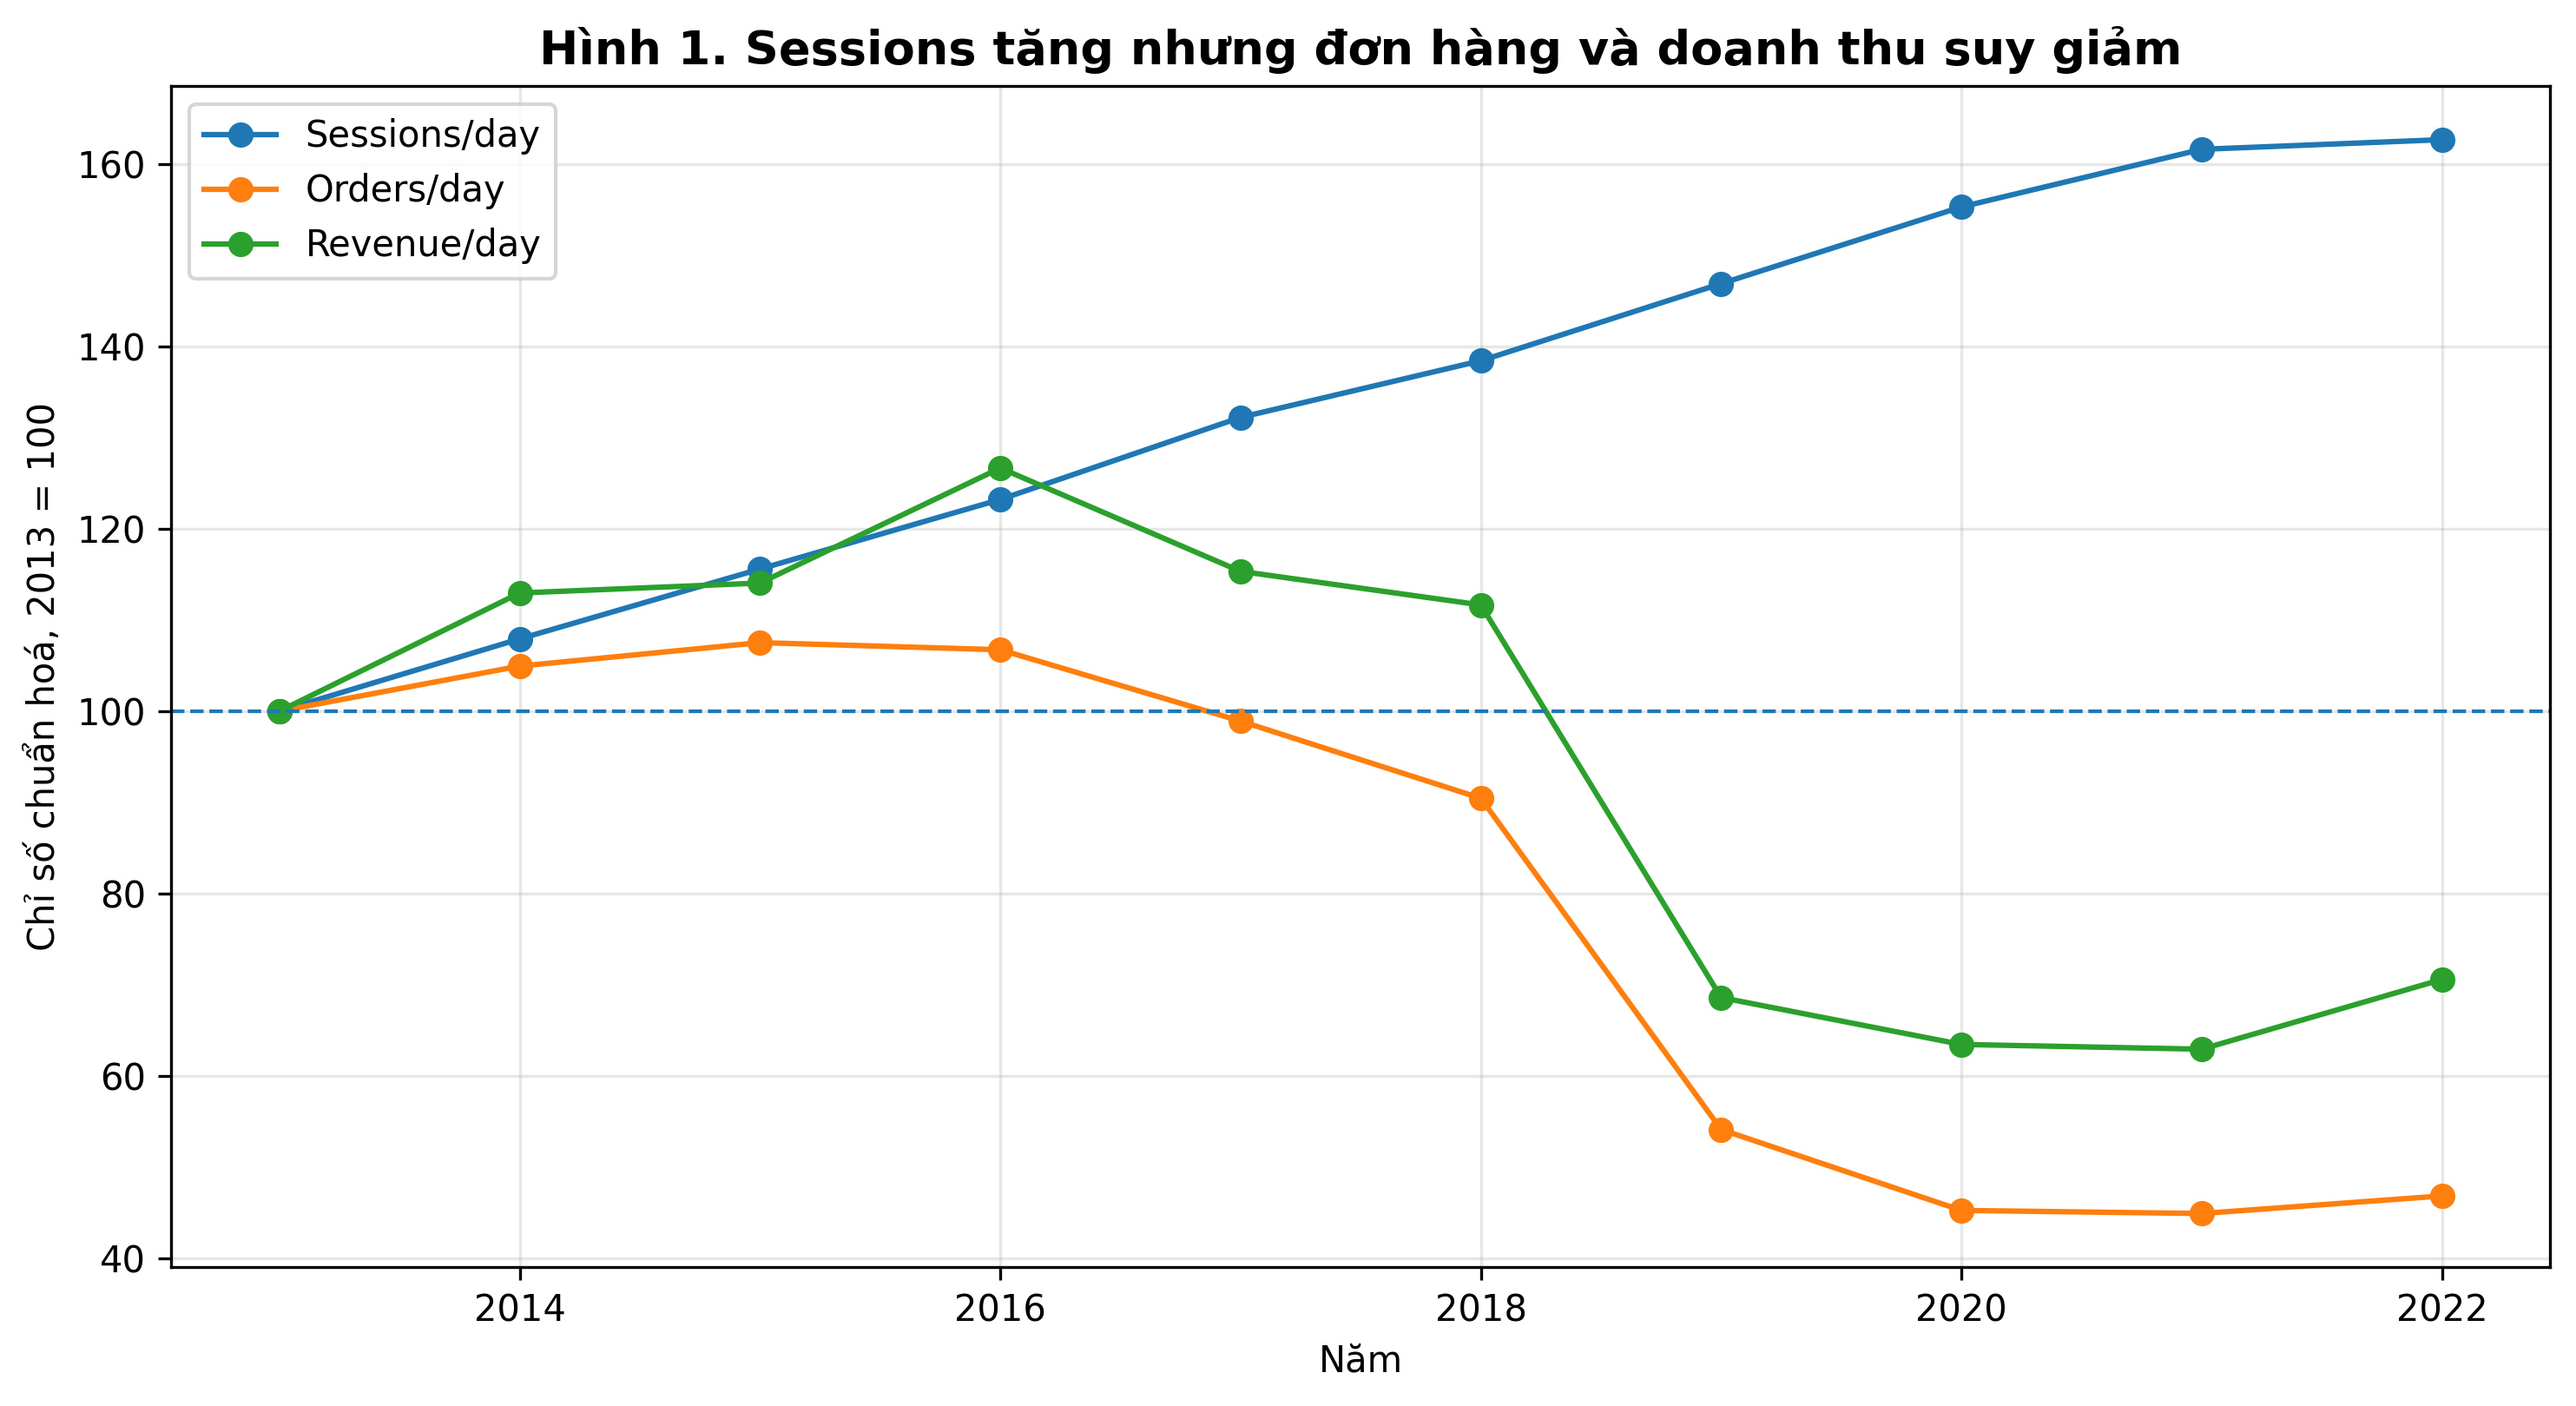
\includegraphics[width=\linewidth]{img/fig01_yearly_index.png}
    \caption{Sessions, orders và revenue/day, chuẩn hoá 2013 = 100.}
    \label{fig:yearly-index}
\end{minipage}
\hfill
\begin{minipage}{0.48\linewidth}
    \centering
    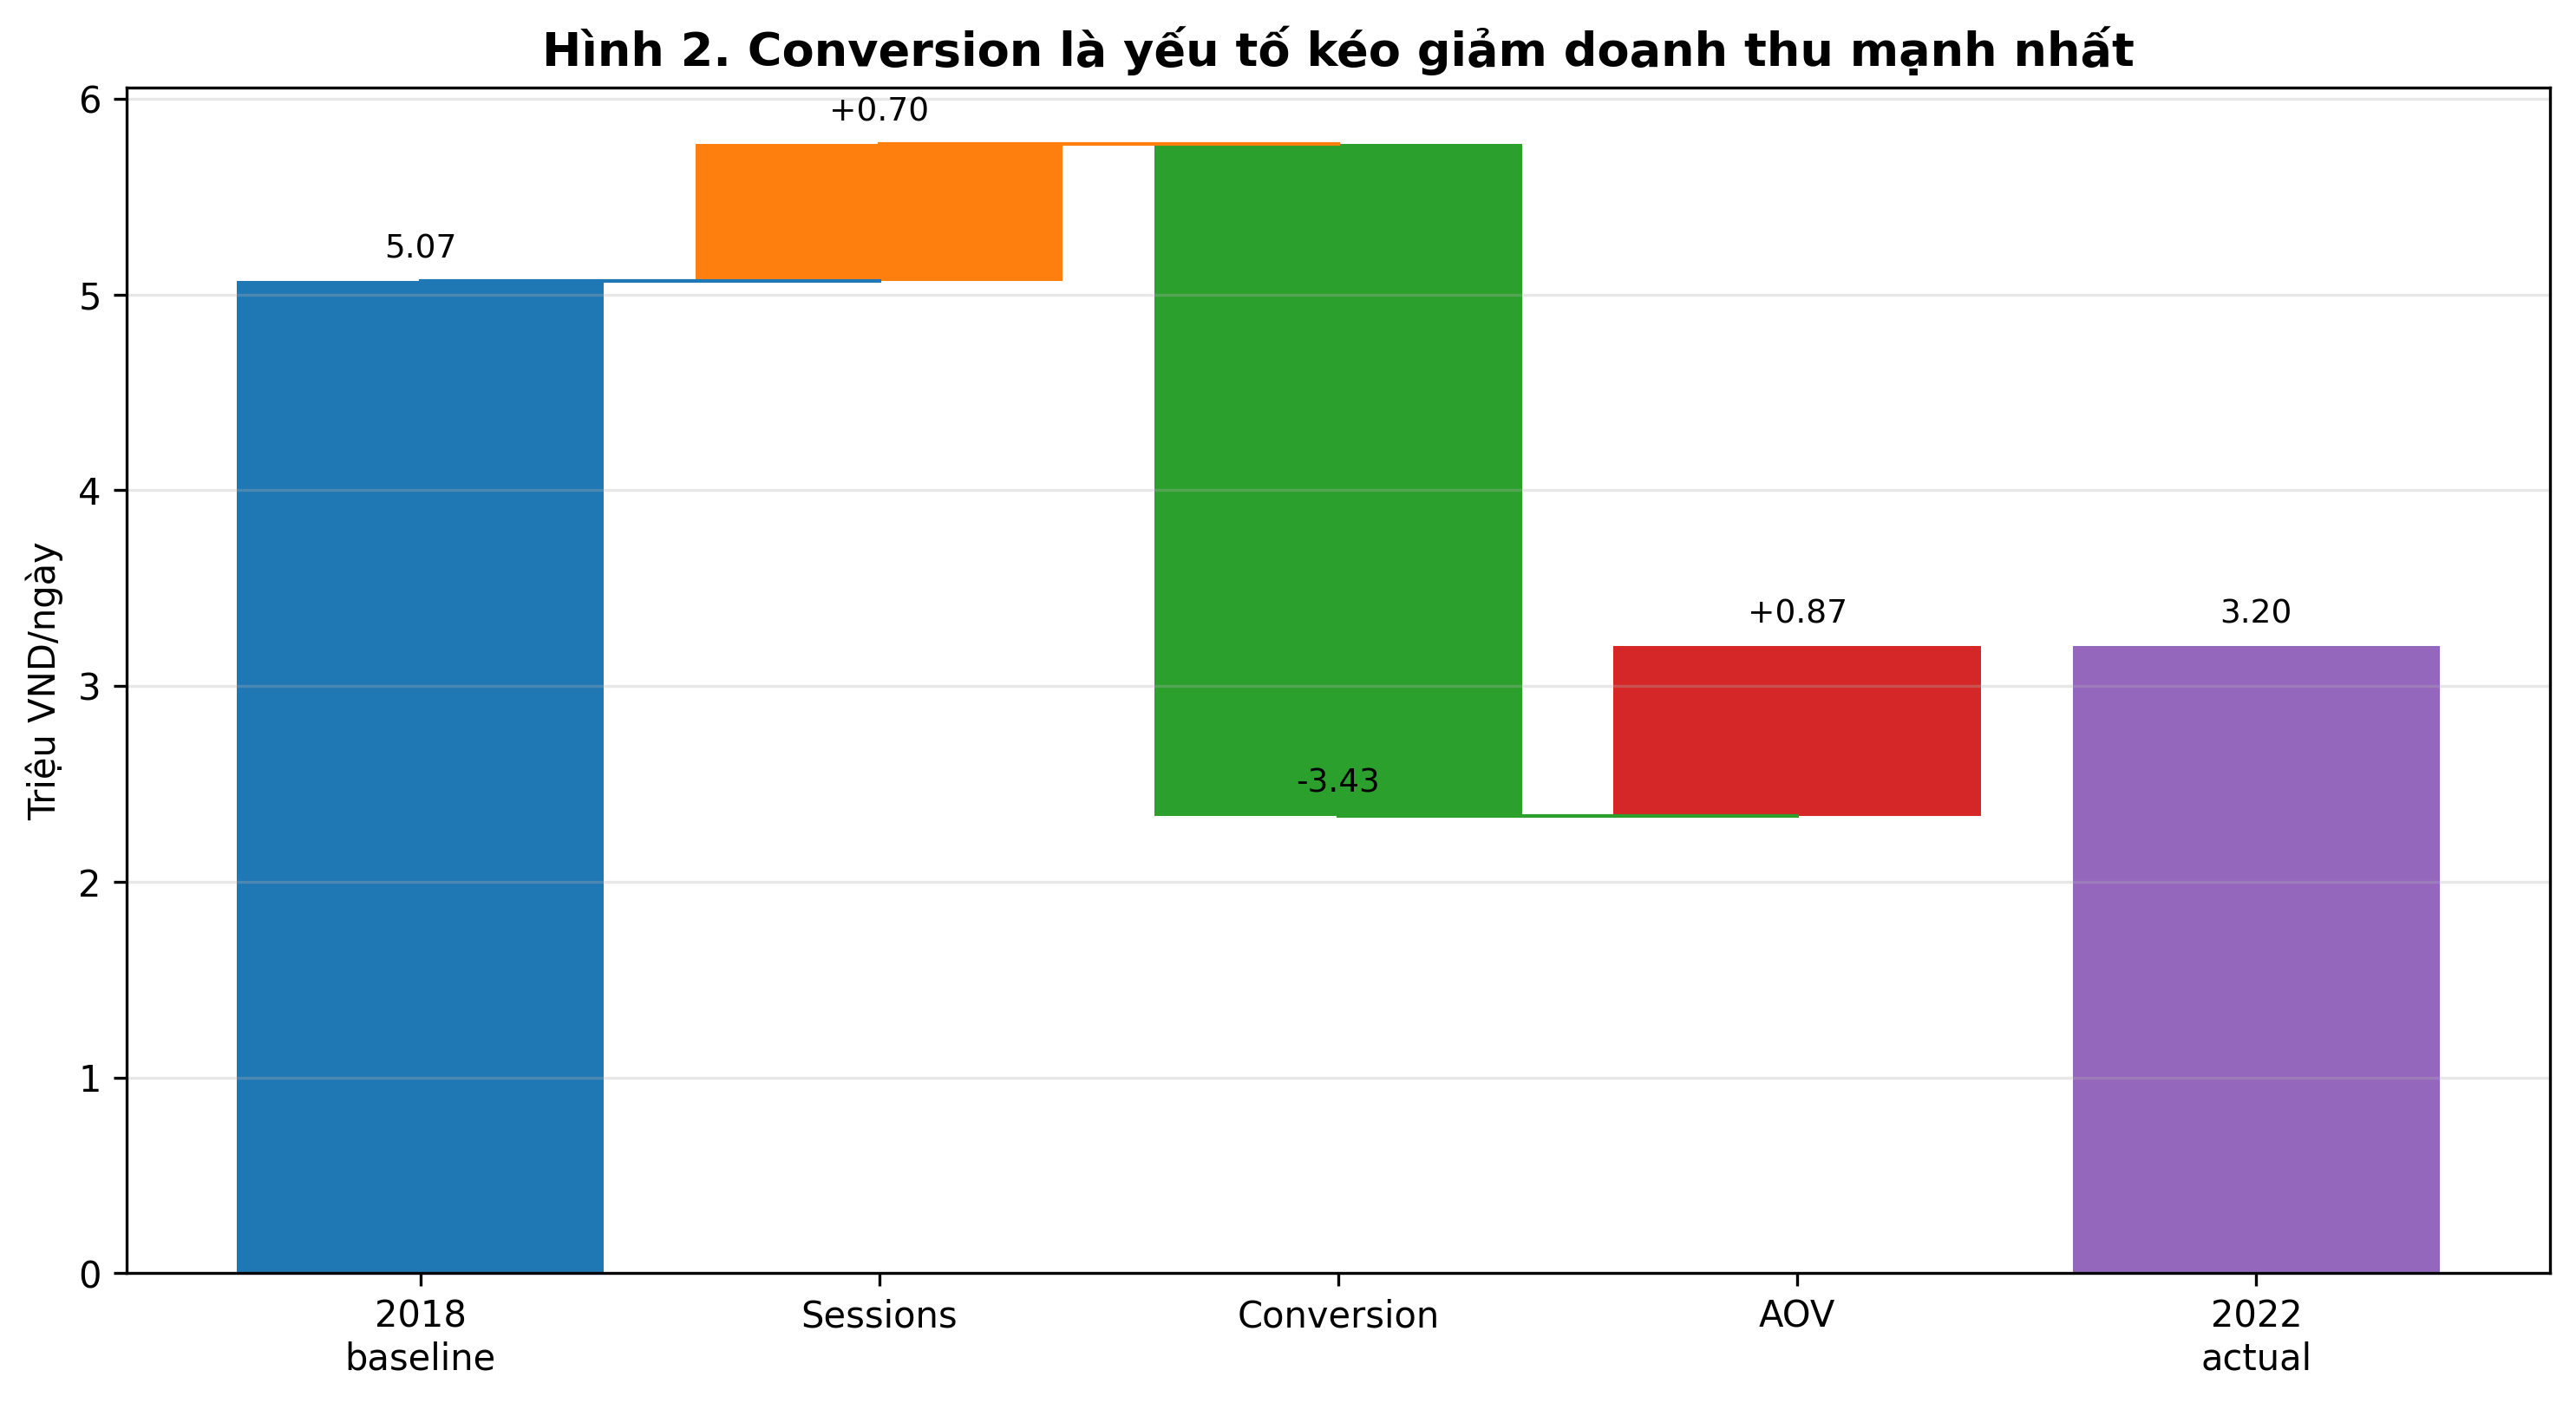
\includegraphics[width=\linewidth]{img/fig02.png}
    \caption{Phân rã doanh thu/ngày giai đoạn 2018--2022.}
    \label{fig:waterfall}
\end{minipage}
\end{figure}

Phân rã thay đổi doanh thu/ngày giữa 2018 và 2022 cho thấy số phiên truy cập đóng góp khoảng
$+0{,}70$ triệu VND/ngày, giá trị trung bình mỗi đơn hàng đóng góp $+0{,}87$ triệu VND/ngày, trong
khi tỷ lệ chuyển đổi kéo giảm khoảng $3{,}43$ triệu VND/ngày. Tổng hợp lại, doanh thu/ngày năm 2022
thấp hơn năm 2018 khoảng $1{,}86$ triệu VND.

Vì vậy, trước khi kéo thêm người dùng mới, doanh nghiệp nên rà soát lại hành trình mua hàng, nhất là
trang sản phẩm, giỏ hàng, phí vận chuyển và bước thanh toán.

\subsection{Mùa bán hàng tốt không chỉ nhìn ở doanh thu}

Phân tích mùa vụ cho thấy doanh thu cao chưa chắc đồng nghĩa với hiệu quả tốt. Quý II đóng góp
$37{,}8\%$ doanh thu năm nhưng tạo ra $48{,}3\%$ lợi nhuận gộp, với biên lợi nhuận gộp
$17{,}2\%$ và tỷ lệ ngày khuyến mại chỉ $27{,}5\%$. Ngược lại, Quý III đóng góp $25{,}0\%$
doanh thu nhưng chỉ tạo ra $11{,}3\%$ lợi nhuận gộp; biên lợi nhuận gộp còn $6{,}1\%$, trong khi
tỷ lệ ngày khuyến mại lên tới $75{,}4\%$.

Ở cấp độ tháng, tháng 5 hiệu quả nhất với doanh thu/ngày khoảng 6,58 triệu VND, biên lợi nhuận gộp
$19{,}9\%$ và không ghi nhận ngày khuyến mại. Tháng 8 là điểm yếu rõ nhất khi biên lợi nhuận gộp
xuống $-8{,}3\%$ và lợi nhuận gộp/ngày âm nhẹ. Tháng 12 có tỷ lệ chuyển đổi cao, $0{,}92\%$, nhưng
giá trị trung bình mỗi đơn chỉ 18.261 VND và biên lợi nhuận gộp chỉ $0{,}7\%$.


\begin{figure}[H]
\centering
\begin{minipage}{0.48\linewidth}
    \centering
    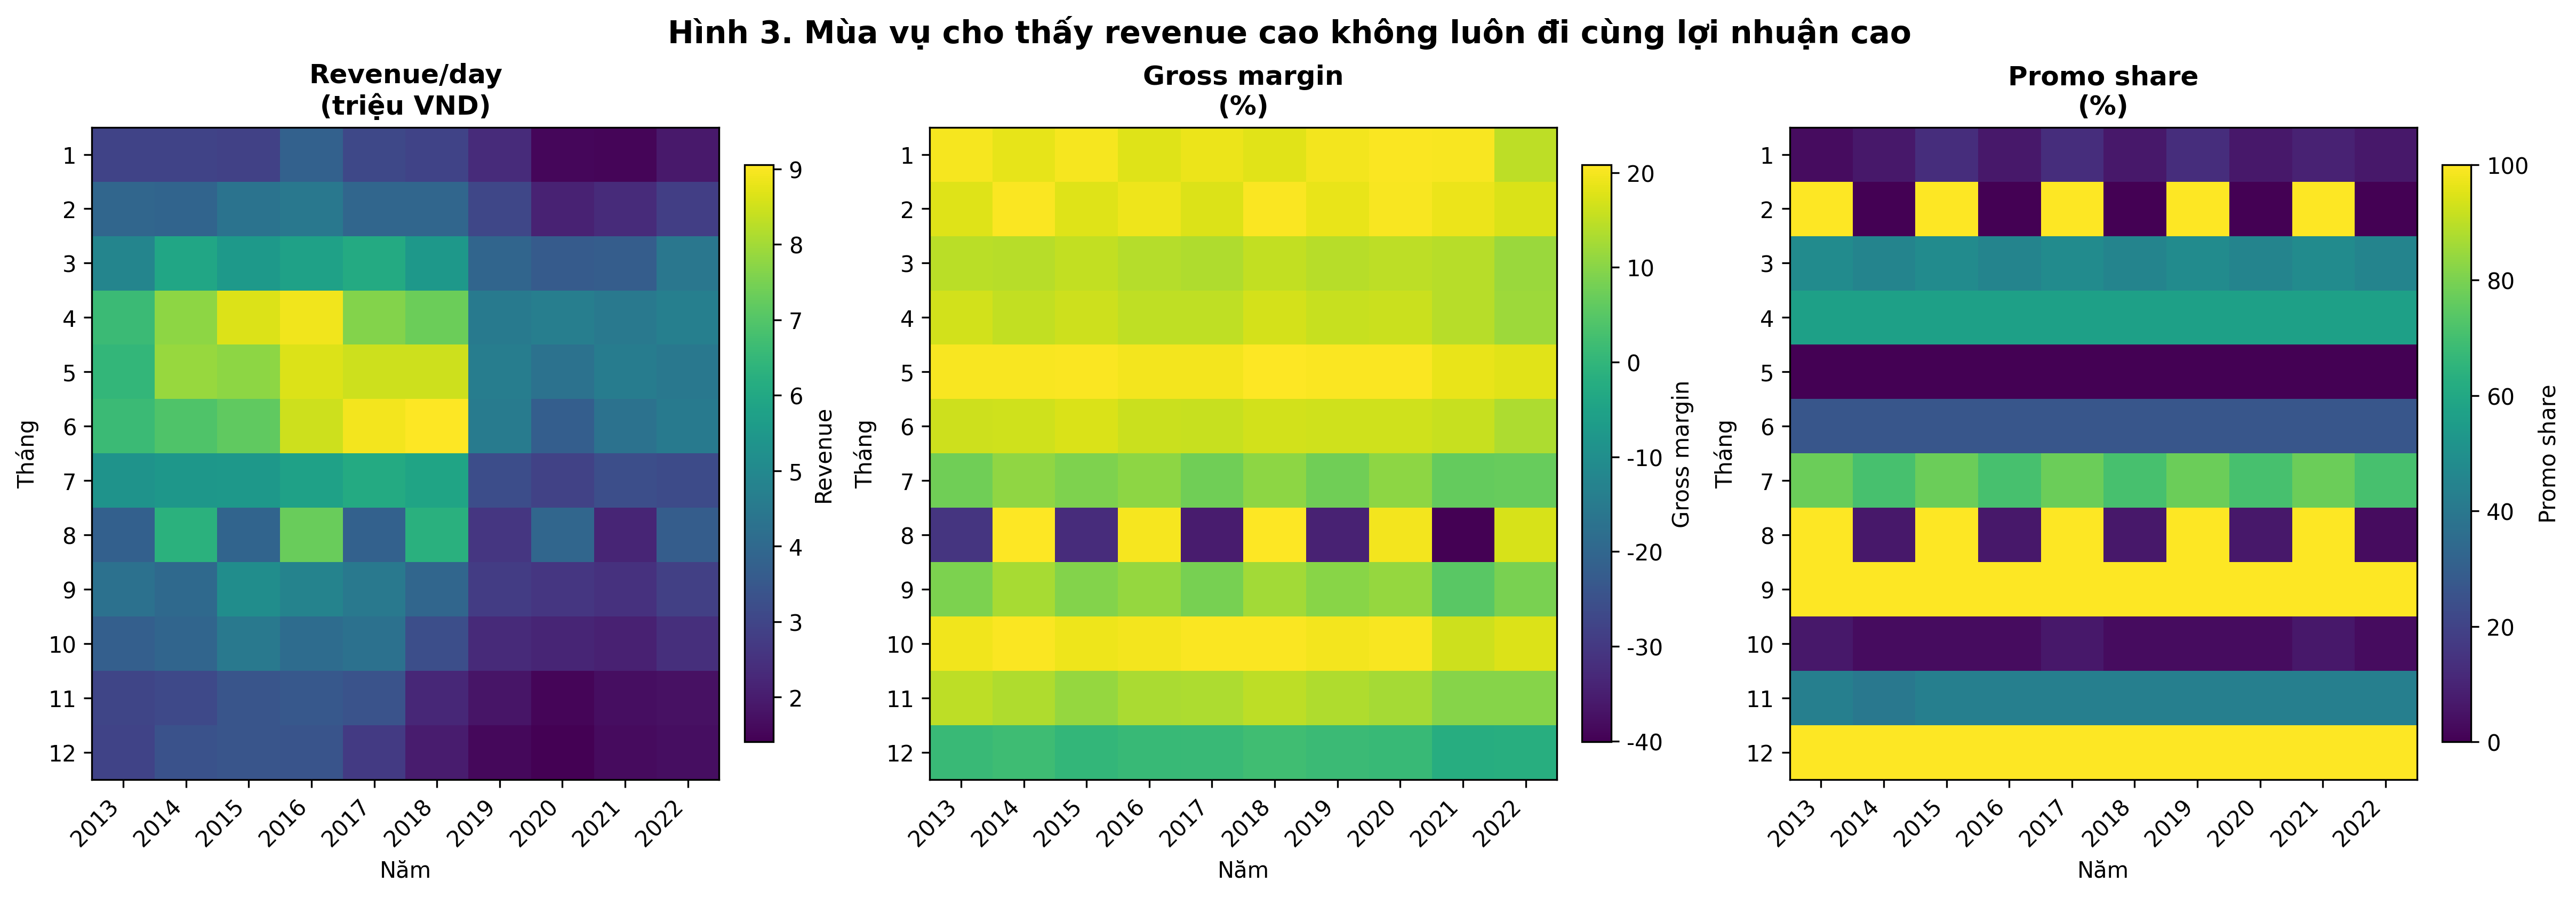
\includegraphics[width=\linewidth]{img/fig03.png}
        \caption{}
    \label{fig:yearly-index}
\end{minipage}
\hfill
\begin{minipage}{0.48\linewidth}
    \centering
    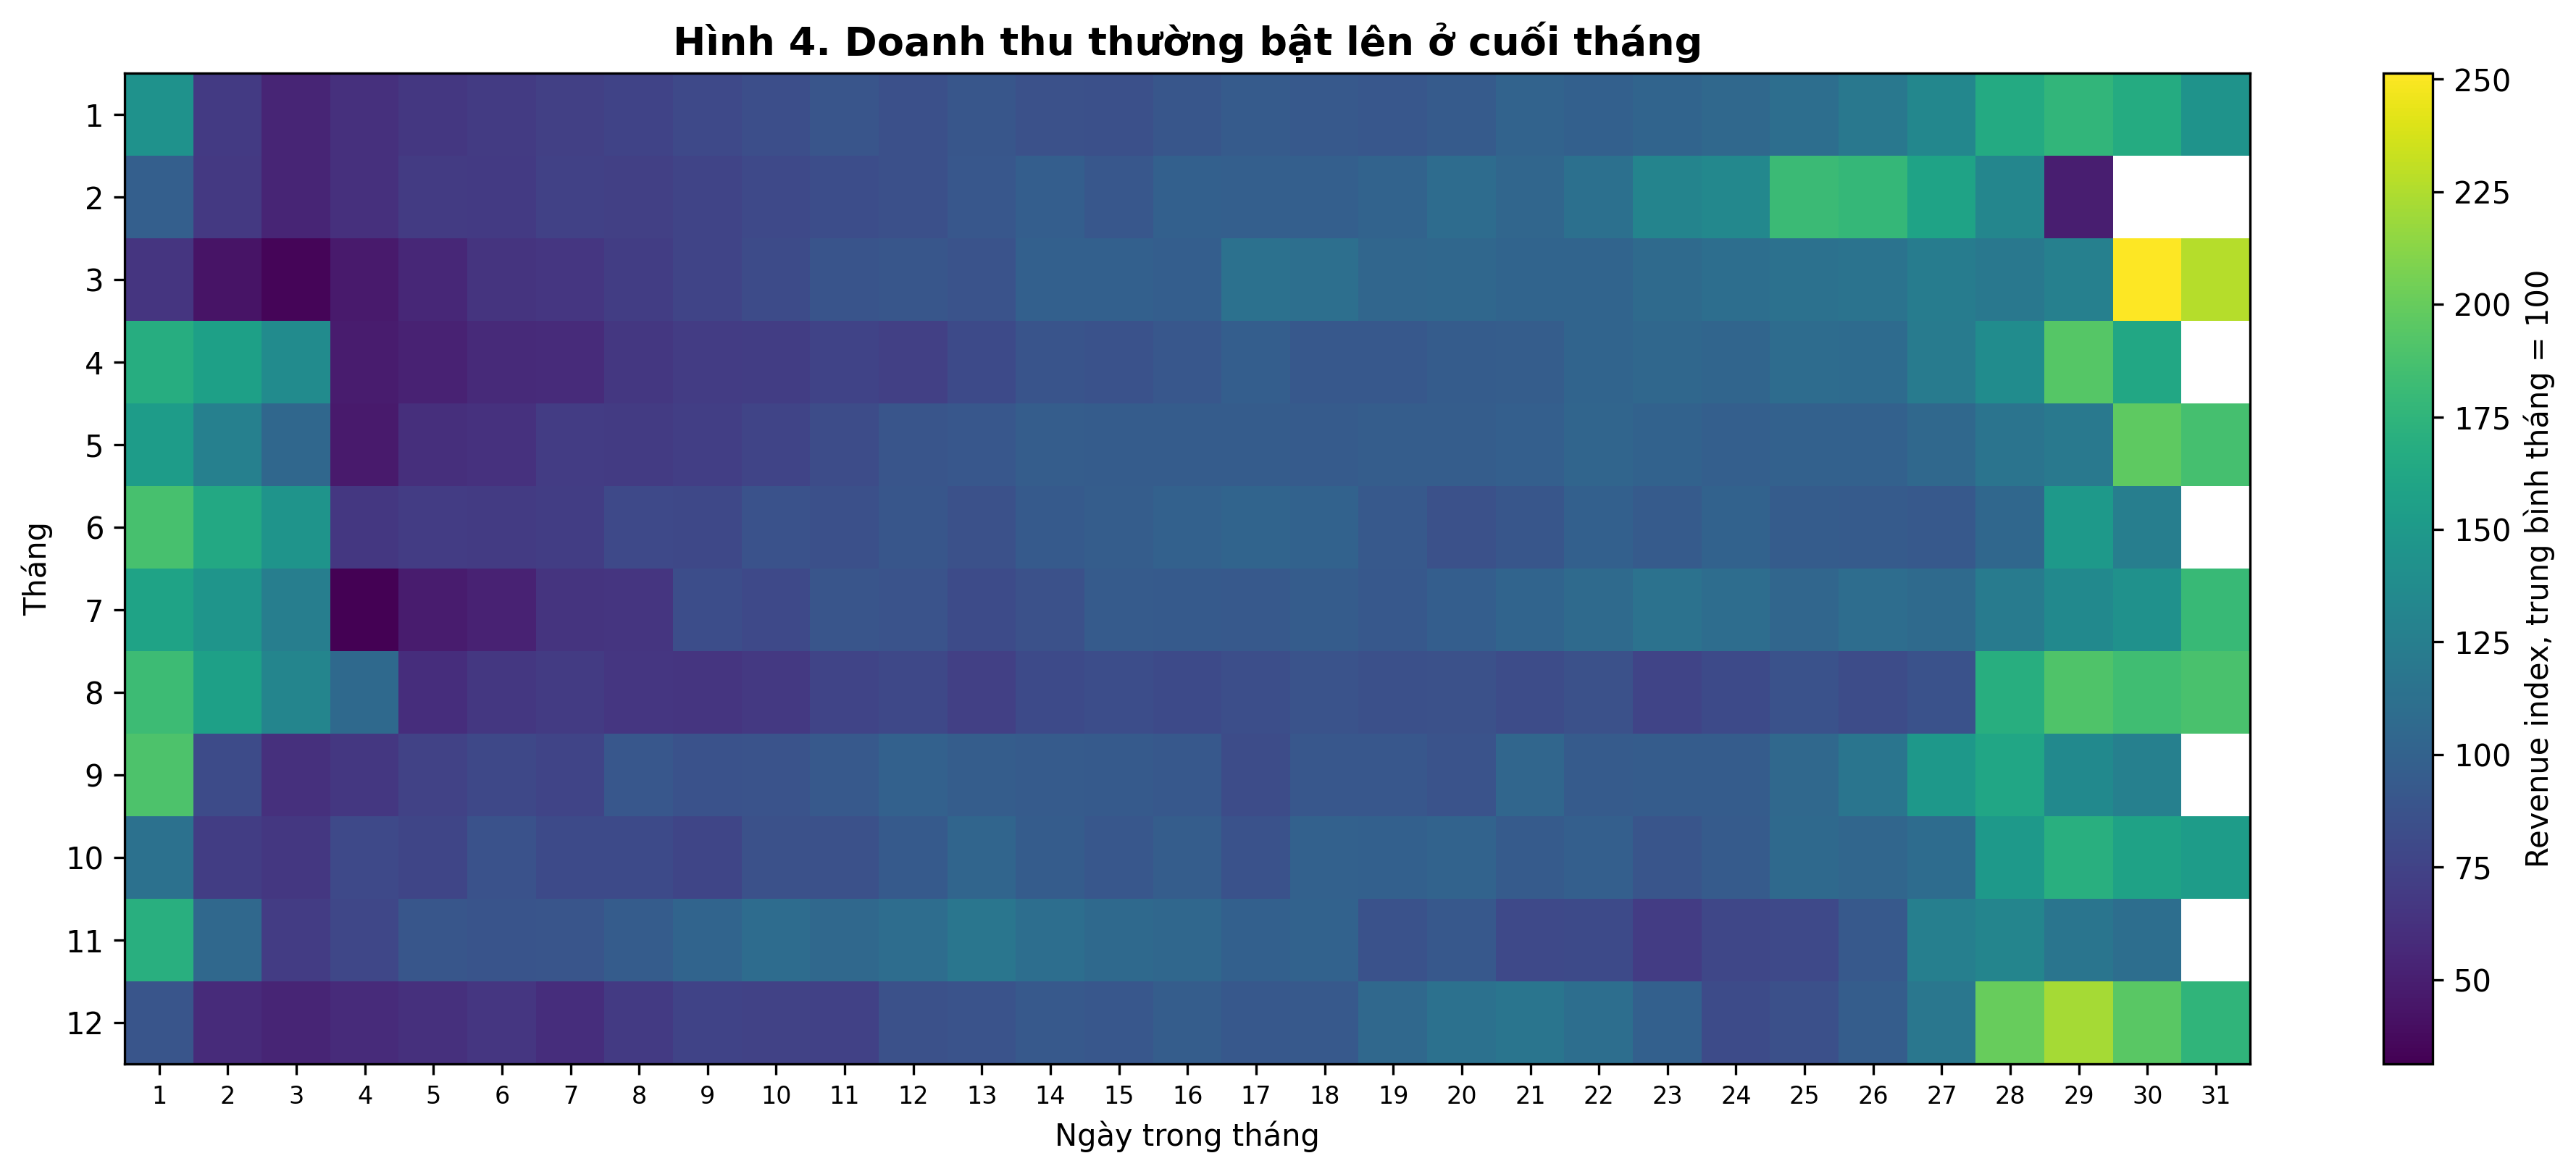
\includegraphics[width=\linewidth]{img/fig04.png}
    \caption{}
    \label{fig:waterfall}
\end{minipage}
\end{figure}


Một mùa bán hàng tốt cần tạo ra cả doanh thu, lợi nhuận gộp và biên lợi nhuận đủ ổn. Điều này phù
hợp với các nghiên cứu về khuyến mại: khuyến mại có thể giúp tăng lượng bán, nhưng không tự động đảm
bảo tăng lợi nhuận \cite{blattberg1990sales}.

\subsection{Cuối tháng là thời điểm người mua dễ ra quyết định hơn}

Nhóm ngày 28--31 đạt doanh thu/ngày 6,79 triệu VND, cao hơn giữa tháng $77{,}1\%$, trong khi số
phiên truy cập gần như không đổi: 25.053 so với 25.051 phiên/ngày. Khác biệt chính nằm ở tỷ lệ
chuyển đổi: cuối tháng đạt $1{,}24\%$, còn giữa tháng chỉ $0{,}65\%$, tức tăng khoảng $90{,}0\%$.
Giá trị trung bình mỗi đơn hàng cuối tháng lại thấp hơn khoảng $5{,}5\%$, cho thấy người dùng dễ ra
quyết định mua hơn chứ không mua đơn lớn hơn.

Dữ liệu tổng hợp theo ngày chưa đủ để khẳng định nguyên nhân như ngày nhận lương hay lịch thanh toán.
Tuy vậy, các nghiên cứu về chu kỳ nhận thu nhập cho thấy chi tiêu thường thay đổi quanh thời điểm
nhận tiền định kỳ \cite{stephens2003third,stephens2006paycheck}. Do đó, nhóm ngày 27--31 là cửa sổ
đáng khai thác cho nhắc giỏ hàng, chăm sóc lại khách cũ, tiếp thị lại hoặc ưu đãi theo ngưỡng.

\subsection{Khuyến mại giúp tăng số đơn, nhưng làm mỏng biên lợi nhuận}

Ngày có khuyến mại có số đơn/ngày cao hơn $8{,}5\%$ và tỷ lệ chuyển đổi cao hơn $15{,}0\%$. Tuy
nhiên, doanh thu/ngày thấp hơn $12{,}6\%$, giá trị trung bình mỗi đơn hàng thấp hơn $19{,}7\%$,
biên lợi nhuận gộp giảm 16,3 điểm phần trăm và lợi nhuận gộp/ngày giảm từ 0,91 triệu xuống
0,20 triệu VND.

Khi kiểm soát theo năm, tháng và ngày trong tuần, khuyến mại vẫn gắn với $+18{,}3\%$ số đơn, nhưng
đi cùng $-17{,}8\%$ giá trị trung bình mỗi đơn, $-2{,}7\%$ doanh thu và $-16{,}0$ điểm phần trăm
biên lợi nhuận gộp. Nói ngắn gọn, khuyến mại có tác dụng kéo đơn, nhưng cách làm hiện tại đang làm
mỏng biên lợi nhuận quá mạnh. Doanh nghiệp nên ưu tiên combo, ưu đãi theo ngưỡng chi tiêu, bán kèm
trong giỏ hàng hoặc ưu đãi cho nhóm khách có khả năng mua lại cao.

\begin{figure}[H]
\centering
\begin{minipage}{0.48\linewidth}
    \centering
    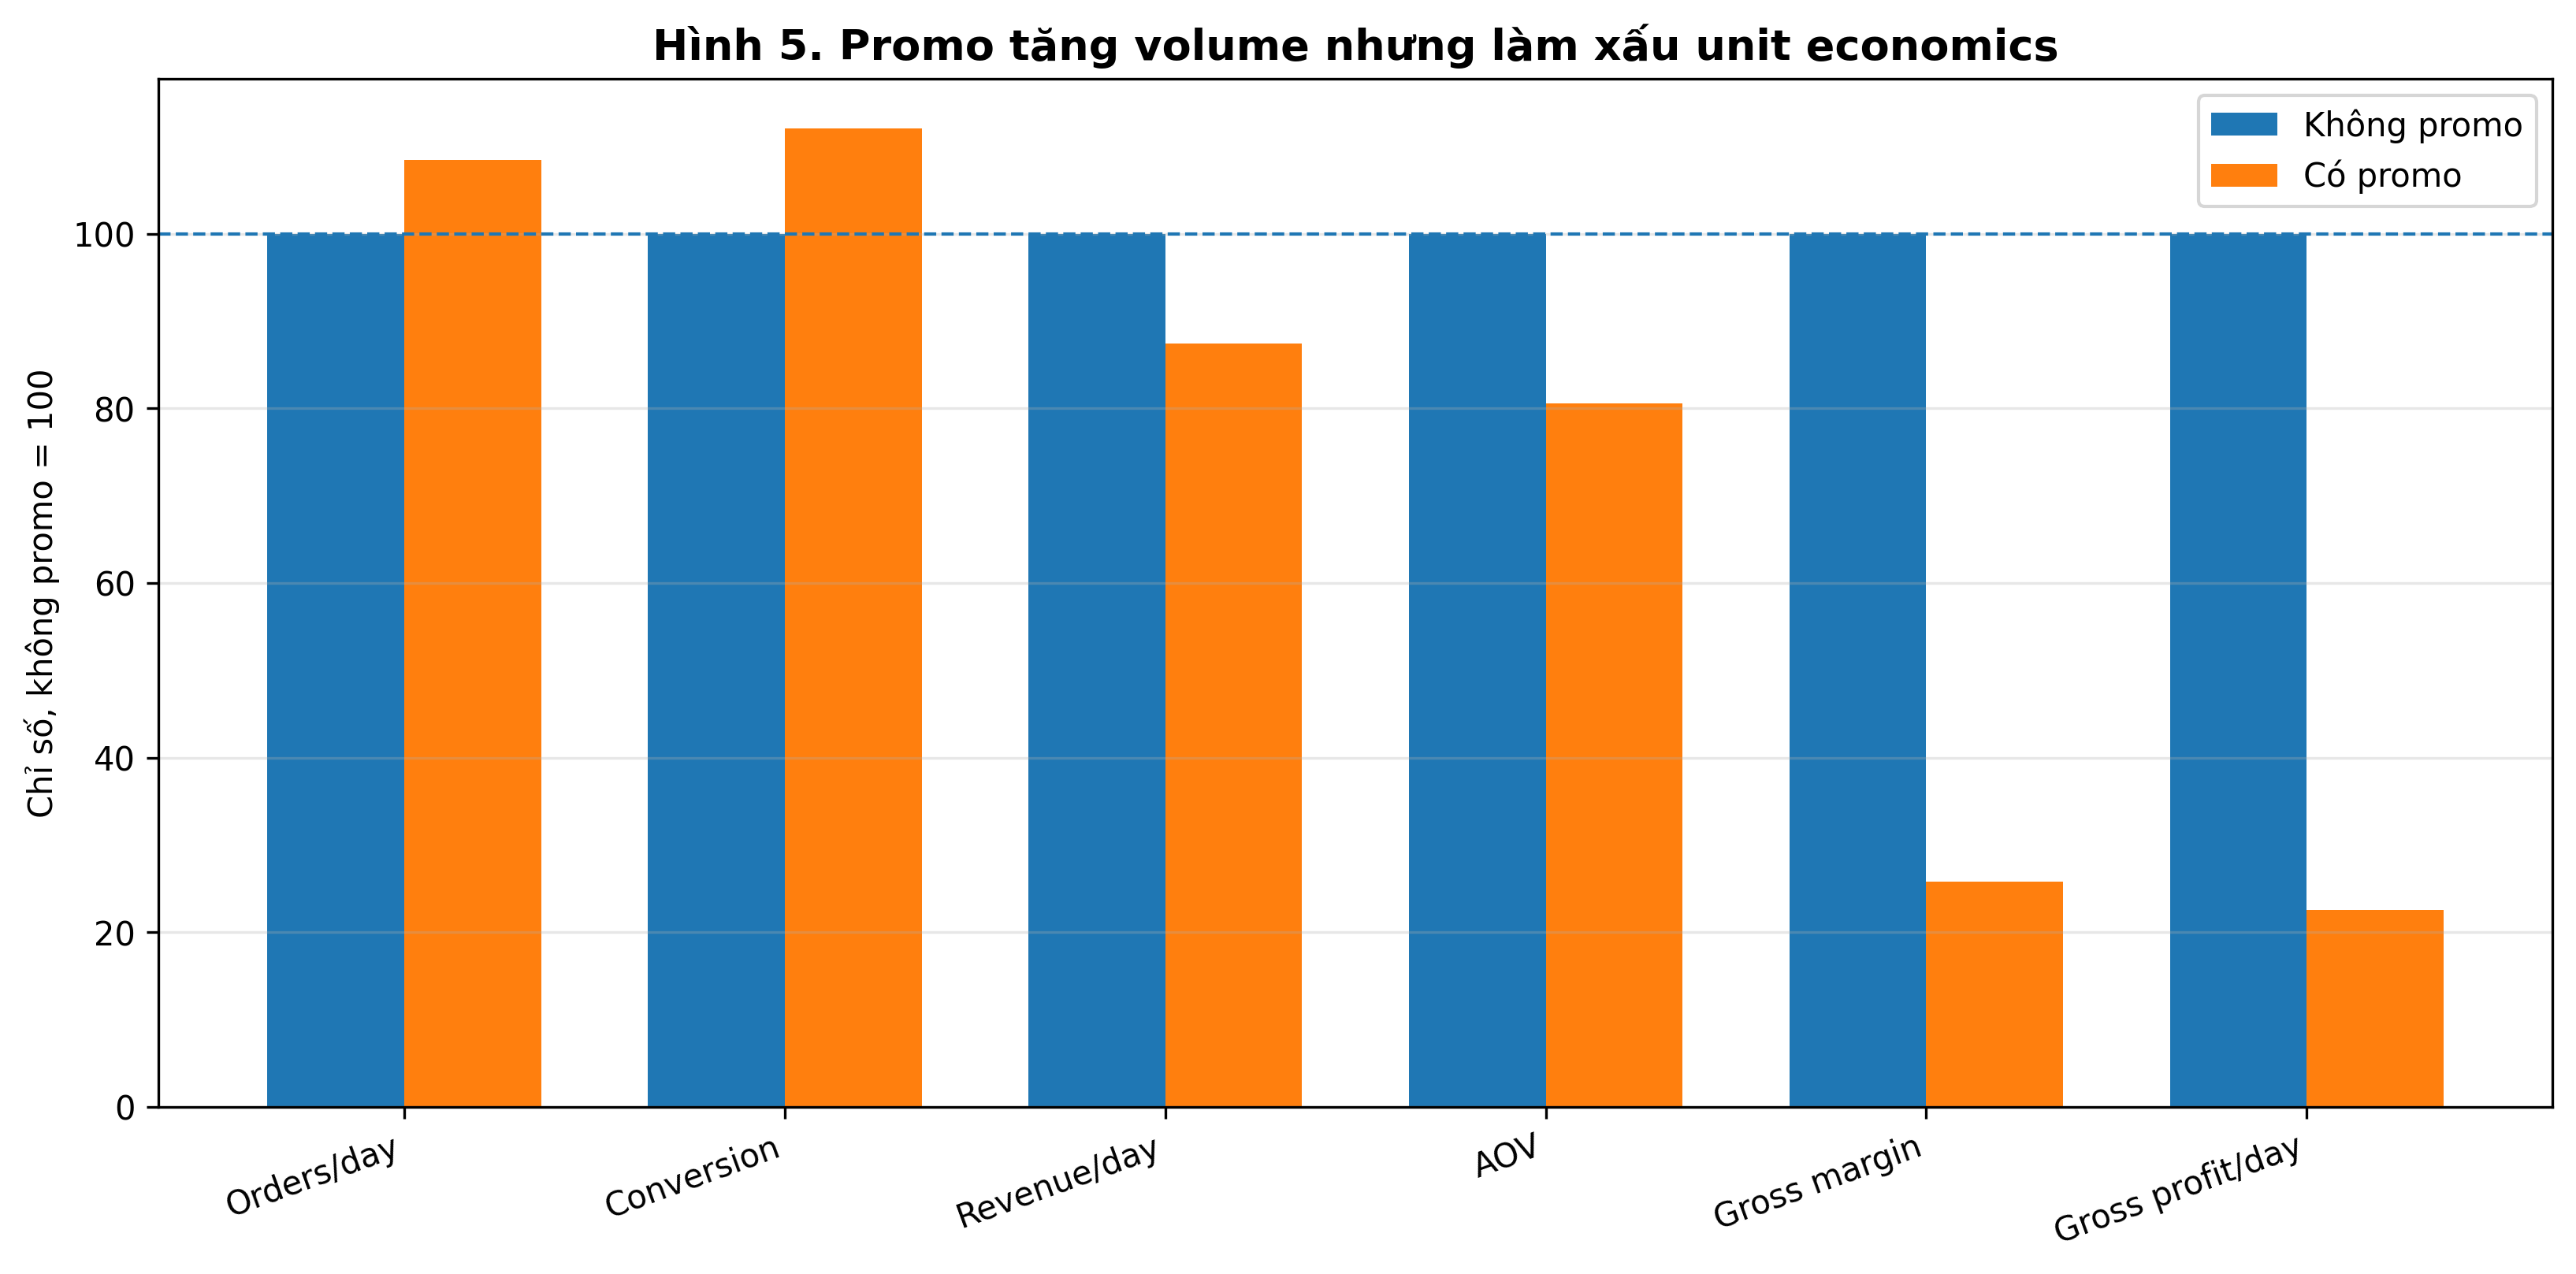
\includegraphics[width=\linewidth]{img/fig05.png}
    \caption{So sánh ngày có và không có khuyến mại.}
    \label{fig:promo}
\end{minipage}
\hfill
\begin{minipage}{0.48\linewidth}
    \centering
    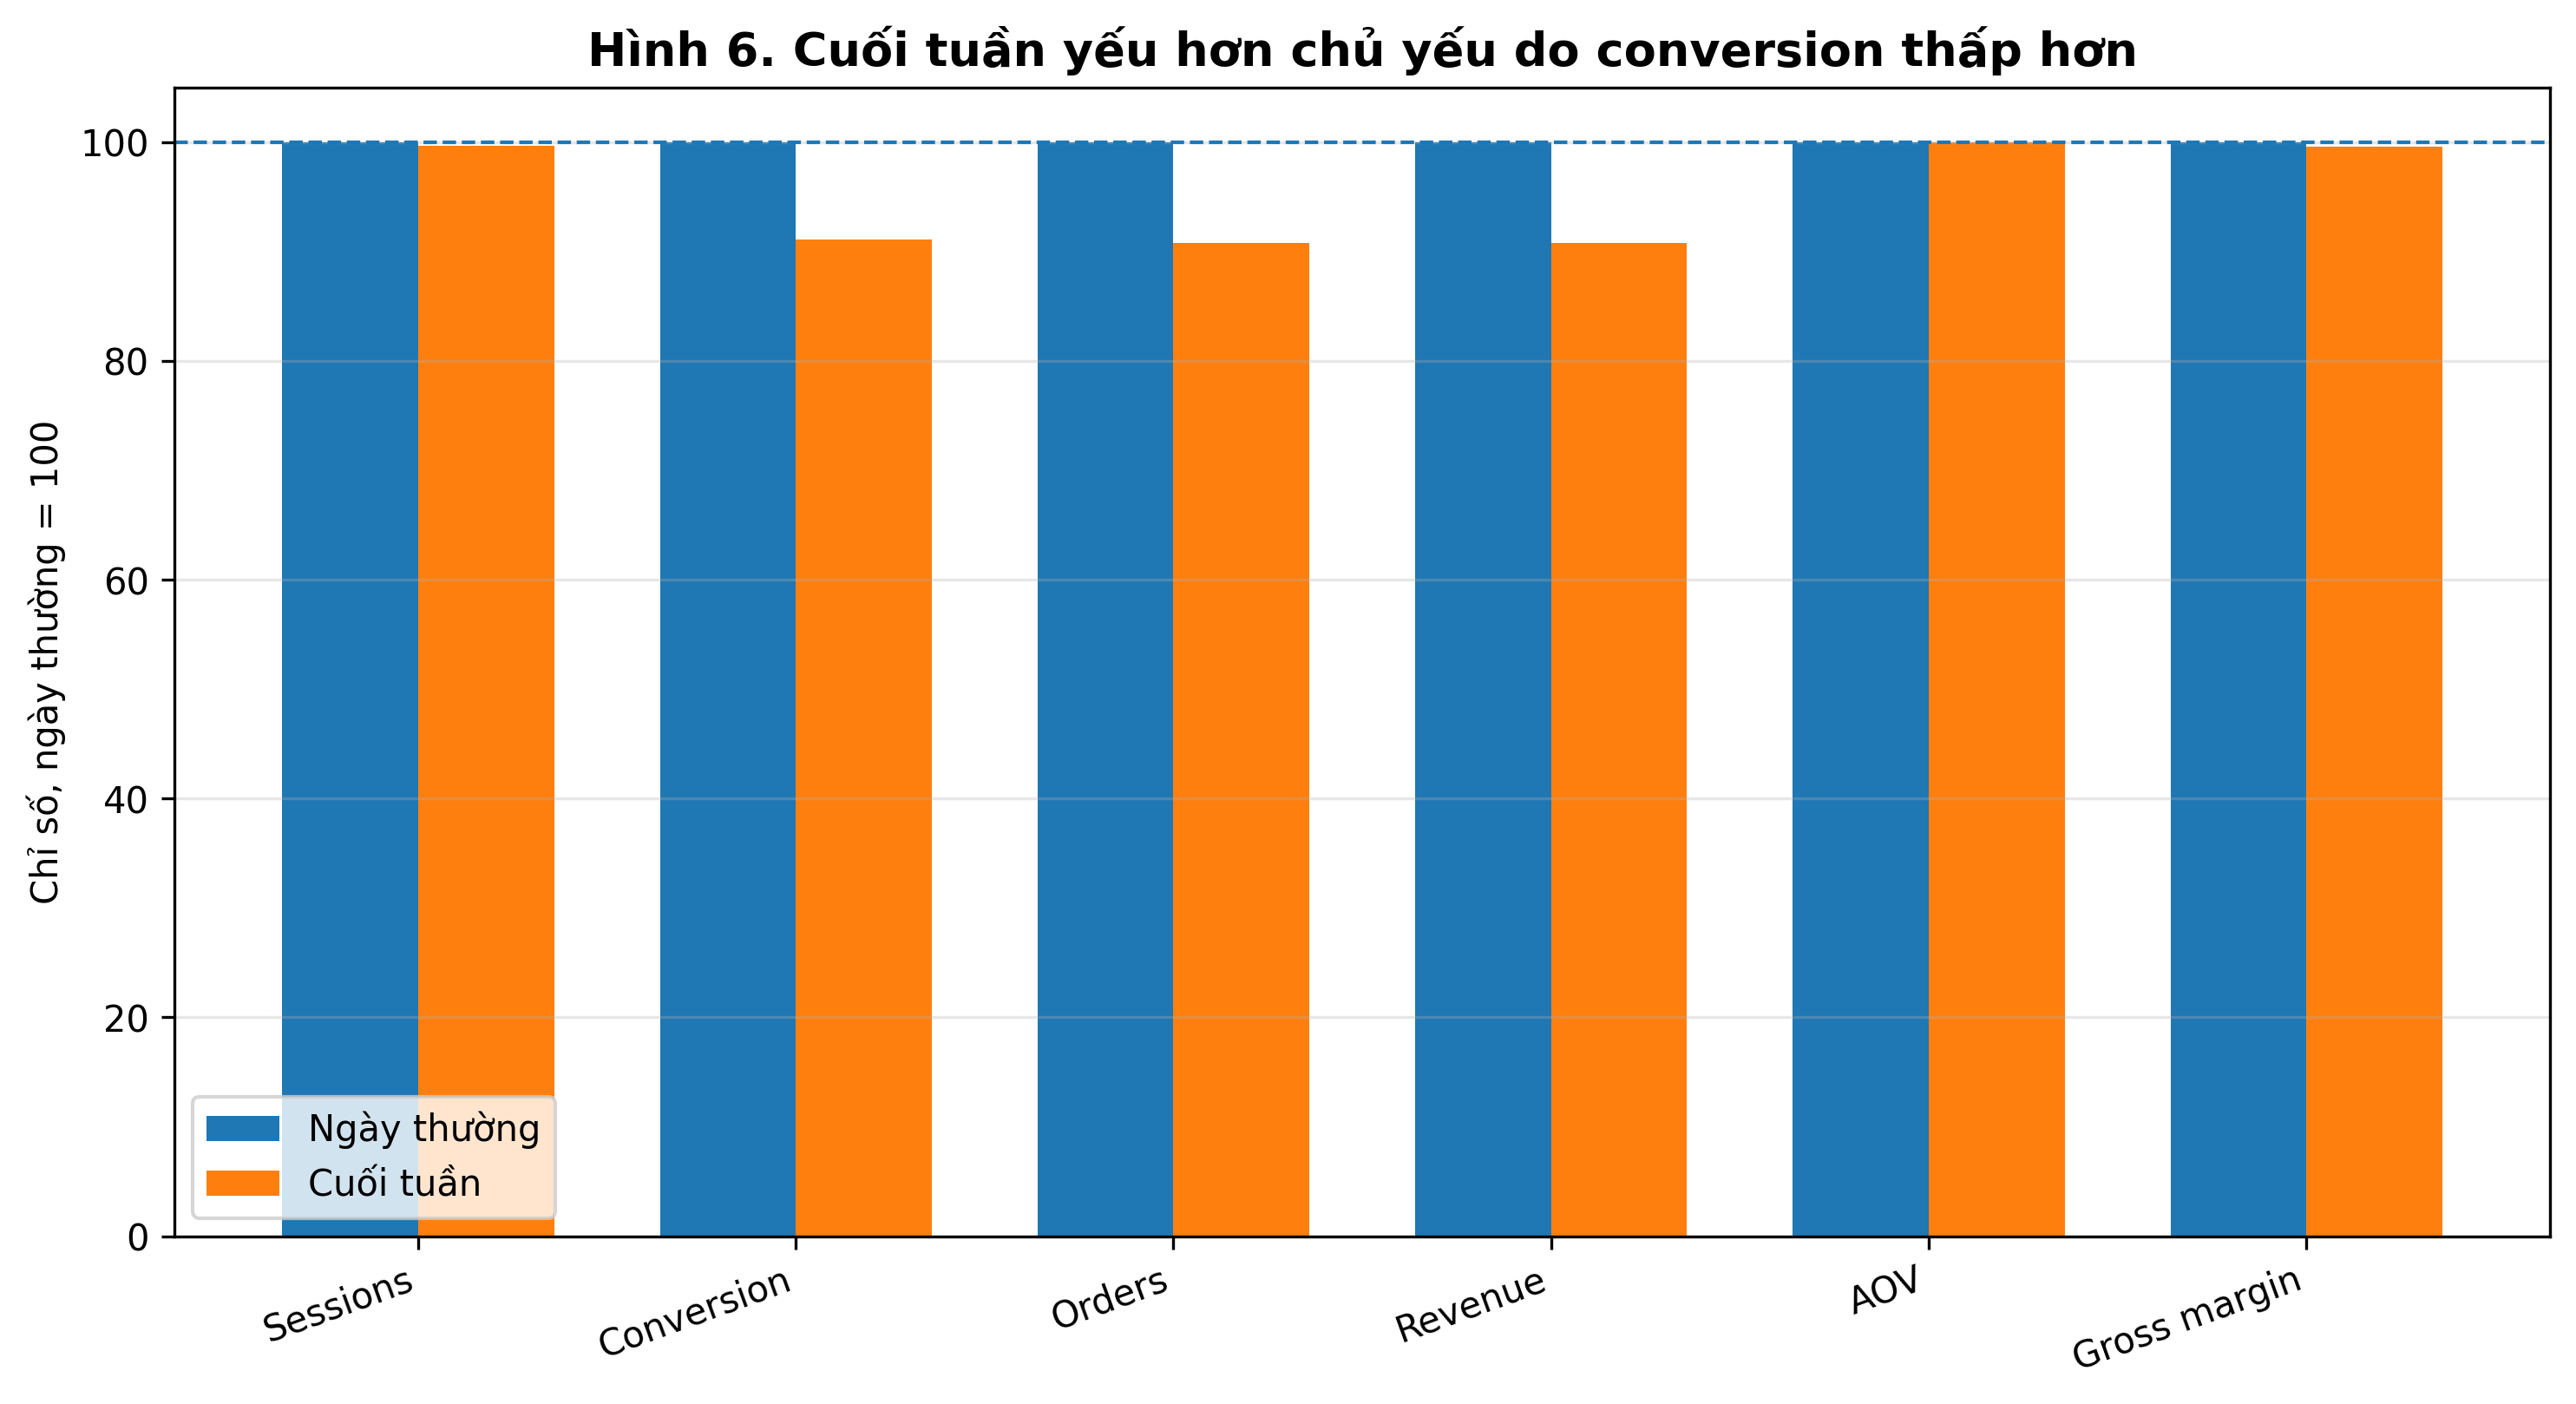
\includegraphics[width=\linewidth]{img/fig06.png}
    \caption{So sánh ngày thường và cuối tuần.}
    \label{fig:weekday-weekend}
\end{minipage}
\end{figure}

Cuối tuần cũng kém hiệu quả hơn ngày thường: doanh thu/ngày thấp hơn khoảng $9{,}2\%$, số phiên truy
cập chỉ thấp hơn $0{,}3\%$, giá trị trung bình mỗi đơn gần như không khác biệt \((+0{,}1\%)\), còn
tỷ lệ chuyển đổi thấp hơn $7{,}2\%$. Vì vậy, cuối tuần phù hợp hơn cho nội dung khám phá, nuôi dưỡng
nhu cầu hoặc nhắc lại thương hiệu.

\subsection{Cải thiện tỷ lệ chuyển đổi là đòn bẩy rõ nhất}

Nếu giữ nguyên số phiên truy cập và giá trị trung bình mỗi đơn hàng của năm 2022, chỉ thay đổi tỷ lệ
chuyển đổi, doanh thu thay đổi rất rõ. Thực tế 2022, tỷ lệ chuyển đổi đạt $0{,}33\%$ và doanh thu
năm là 1,170 tỷ VND. Nếu tăng lên $0{,}40\%$, số đơn hàng ước đạt 44.255 đơn, doanh thu đạt
$1{,}438$ tỷ VND, tăng thêm 268,1 triệu VND. Nếu đạt $0{,}50\%$, số đơn hàng ước đạt 55.318 đơn,
doanh thu đạt $1{,}797$ tỷ VND, tăng thêm 627,5 triệu VND. Mức $0{,}50\%$ vẫn thấp hơn $0{,}74\%$
của năm 2018, nên đây là mục tiêu có cơ sở lịch sử.

\begin{figure}[H]
\centering
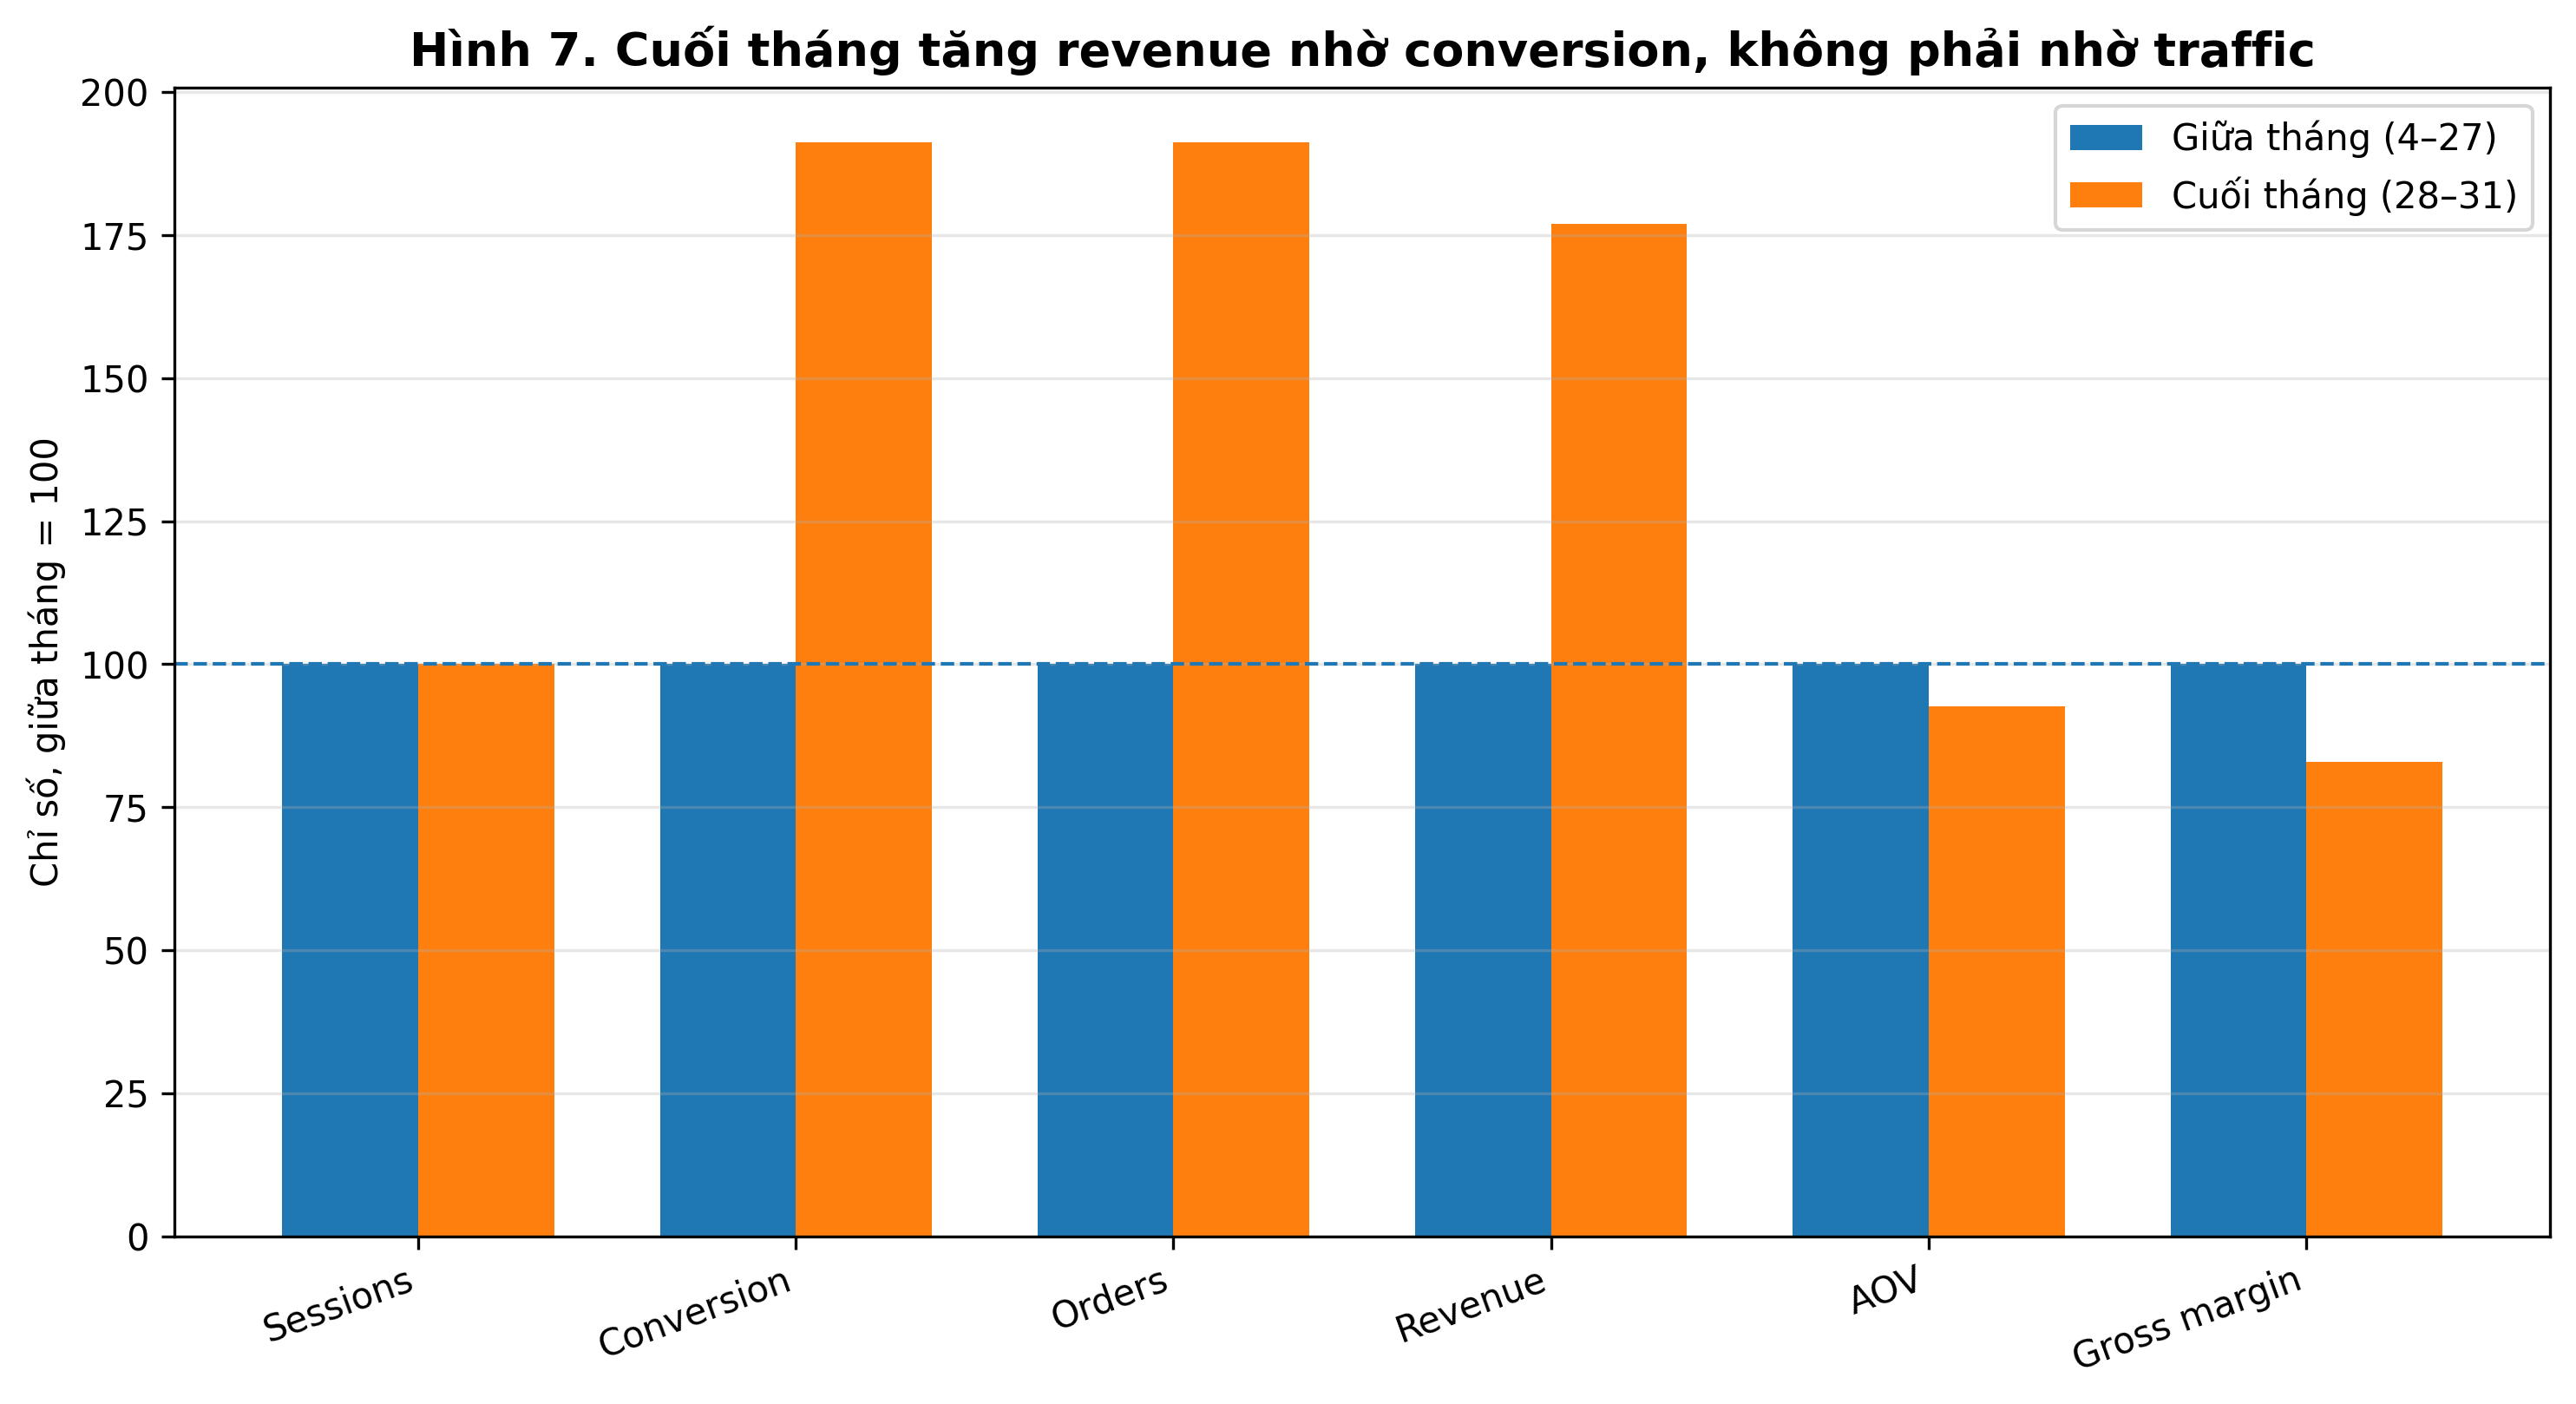
\includegraphics[width=0.7\linewidth]{img/fig07.png}
\caption{Kịch bản doanh thu nếu cải thiện tỷ lệ chuyển đổi từ mặt bằng năm 2022.}
\label{fig:scenario}
\end{figure}

Do đó, hướng ưu tiên ngắn hạn nên là tối ưu tỷ lệ chuyển đổi trước khi mở rộng hoạt động thu hút
lượt truy cập mới. Các thay đổi ở trang sản phẩm, giỏ hàng, form thanh toán, phí vận chuyển, ngưỡng
miễn phí vận chuyển hoặc nhắc giỏ hàng cuối tháng nên được kiểm định bằng A/B testing thay vì chỉ dựa
vào cảm tính \cite{kohavi2007controlled,kohavi2020trustworthy}.

% =========================================================
\section{Mô hình dự báo doanh thu}

\subsection{Mục tiêu và hướng xây dựng mô hình}

Bài toán yêu cầu dự báo doanh thu theo ngày cho giai đoạn 01/01/2023 đến 01/07/2024. Tập huấn luyện
gồm dữ liệu lịch sử từ 04/07/2012 đến 31/12/2022, khoảng 3.833 ngày quan sát. File nộp cuối cùng gồm
ba cột \texttt{Date}, \texttt{Revenue} và \texttt{COGS}. Vì thước đo đánh giá gồm MAE, RMSE và
$R^2$, mô hình cần ổn định ở mức trung bình và hạn chế sai số lớn ở những ngày doanh thu cao.

Nhóm xây dựng quy trình kết hợp thay vì dùng một mô hình đơn lẻ, vì doanh thu theo ngày vừa có mùa vụ,
vừa chịu ảnh hưởng của khuyến mại, số phiên truy cập, số đơn hàng và các dao động ngắn hạn.

\subsection{Tạo biến đầu vào và mô hình nền}

Biến đầu vào gồm bốn nhóm: thời gian, lịch sử doanh thu, khuyến mại và biến vận hành theo ngày. Từ
\texttt{Date}, mô hình sinh tháng, ngày, thứ trong tuần, ngày trong năm, tuần trong năm, vị trí ngày
trong tháng, cuối tuần và các biến chu kỳ dạng sin--cos. Thông tin khuyến mại được mở rộng theo từng
ngày hiệu lực để tạo \texttt{promo\_count}, \texttt{promo\_discount\_sum} và
\texttt{promo\_discount\_mean}. Một số biến lệch lớn như \texttt{page\_views},
\texttt{order\_count} và \texttt{total\_discount} được biến đổi bằng $\log(1+x)$.

Quy trình bắt đầu bằng mô hình nền theo lịch sử. Với mỗi cặp tháng--ngày, mô hình lấy trung vị doanh
thu và COGS trong quá khứ:
\[
BaseRevenue_{m,d}=median(Revenue_t \mid month_t=m, day_t=d).
\]
Trung vị ít bị kéo lệch bởi các ngày bất thường. Sau đó, mô hình nền được hiệu chỉnh theo thứ trong
tuần để phản ánh khác biệt giữa ngày thường và cuối tuần.

\subsection{Kết hợp mô hình học máy}

Sau mô hình nền, XGBoost học quan hệ phi tuyến giữa doanh thu, thời gian, khuyến mại và các biến
rolling. ExtraTrees và Gradient Boosting dự báo phần chênh lệch giữa doanh thu thực tế và mô hình
nền:
\[
ResidualRevenue_t=Revenue_t-BaseRevenue_t.
\]
Nhờ đó, mô hình nền giữ vai trò bám mùa vụ, còn các mô hình học máy xử lý dao động theo ngày như
khuyến mại, số phiên truy cập, số đơn hàng hoặc tổng giảm giá.

Mô hình cuối cùng kết hợp mô hình nền, XGBoost, ExtraTrees, Gradient Boosting, nhánh kiểm tra theo
cấu trúc:
\[
Revenue \approx OrderCount \times AOV,
\]
và một nhánh hiệu chỉnh cục bộ với trọng số 0,060. Nhánh \texttt{order\_count}--AOV giúp dự báo gần
hơn với logic kinh doanh, còn việc trộn nhiều nhánh giúp kết quả ổn định hơn.

\subsection{Xử lý kết quả cuối và kiểm soát rò rỉ dữ liệu}

Revenue và COGS được giới hạn theo các phân vị cao của tập huấn luyện:
\[
Revenue_t \leq Q_{0.997}^{Revenue}, \qquad COGS_t \leq Q_{0.998}^{COGS}.
\]
Nếu COGS lớn hơn Revenue, mô hình điều chỉnh:
\[
COGS_t=0.92\times Revenue_t.
\]
Bước này giúp dự báo hợp lý hơn về mặt kinh doanh và giảm rủi ro tạo sai số lớn, đặc biệt với RMSE.

Toàn bộ quy trình chỉ sử dụng dữ liệu cuộc thi, không dùng dữ liệu ngoài. Các biến thời gian được
sinh trực tiếp từ cột \texttt{Date}; các biến lịch sử như rolling median, mô hình nền và phần sai
lệch còn lại được xây dựng từ tập huấn luyện, không sử dụng doanh thu thực tế của tập test. Các seed
cố định gồm 11, 22, 33, 44, 55, 777, 888 và 2026 để tăng khả năng tái lập.

Nhìn chung, mô hình được thiết kế để vừa bám quy luật lịch sử, vừa phản ánh được các dao động ngắn
hạn trong bài toán doanh thu theo ngày.

% =========================================================
\phantomsection
\addcontentsline{toc}{section}{Tài liệu tham khảo}
\renewcommand{\refname}{Tài liệu tham khảo}
\begin{thebibliography}{99}
\bibitem{davenport2013analytics}
Thomas H. Davenport.
\newblock Analytics 3.0.
\newblock \emph{Harvard Business Review}, December 2013.
\newblock \url{https://hbr.org/2013/12/analytics-30}

\bibitem{kohavi2007controlled}
Ron Kohavi, Randolph M. Henne, and Dan Sommerfield.
\newblock Controlled experiments on the web: Survey and practical guide.
\newblock In \emph{Proceedings of the 13th ACM SIGKDD International Conference on Knowledge Discovery and Data Mining}, pages 959--967, 2007.
\newblock DOI: \url{https://doi.org/10.1145/1281192.1281295}

\bibitem{kohavi2020trustworthy}
Ron Kohavi, Diane Tang, and Ya Xu.
\newblock \emph{Trustworthy Online Controlled Experiments: A Practical Guide to A/B Testing}.
\newblock Cambridge University Press, 2020.
\newblock DOI: \url{https://doi.org/10.1017/9781108653985}

\bibitem{blattberg1990sales}
Robert C. Blattberg and Scott A. Neslin.
\newblock \emph{Sales Promotion: Concepts, Methods, and Strategies}.
\newblock Prentice Hall, 1990.
\newblock ISBN: 9780134423029.

\bibitem{zimmermann2023cro}
Robert Zimmermann and Andreas Auinger.
\newblock Developing a conversion rate optimization framework for digital retailers -- case study.
\newblock \emph{Journal of Marketing Analytics}, 11(2):233--243, 2023.
\newblock DOI: \url{https://doi.org/10.1057/s41270-022-00161-y}

\bibitem{baymard2025checkout}
Baymard Institute.
\newblock Cart \& Checkout Usability Research.
\newblock Baymard Institute Research Overview, accessed 2026.
\newblock \url{https://baymard.com/research/checkout-usability}

\bibitem{baymard2025abandonment}
Christian Holst.
\newblock Reasons for Cart Abandonment -- Why Users Abandon Their Cart.
\newblock Baymard Institute, updated 2025.
\newblock \url{https://baymard.com/blog/ecommerce-checkout-usability-report-and-benchmark}

\bibitem{stephens2003third}
Melvin Stephens Jr.
\newblock ``3rd of tha Month'': Do Social Security Recipients Smooth Consumption Between Checks?
\newblock \emph{American Economic Review}, 93(1):406--422, 2003.
\newblock DOI: \url{https://doi.org/10.1257/000282803321455386}

\bibitem{stephens2006paycheck}
Melvin Stephens Jr.
\newblock Paycheque receipt and the timing of consumption.
\newblock \emph{The Economic Journal}, 116(513):680--701, 2006.
\newblock DOI: \url{https://doi.org/10.1111/j.1468-0297.2006.01106.x}
\end{thebibliography}

\appendix
\section*{Danh mục ký hiệu}
\setcounter{page}{0}
\thispagestyle{empty}
\addcontentsline{toc}{section}{Danh mục ký hiệu}

\begin{table}[H]
\centering
\small
\caption{Ký hiệu và thước đo sử dụng trong báo cáo}
\label{tab:notations}
\begin{tabularx}{\textwidth}{
>{\raggedright\arraybackslash}p{0.18\textwidth}
>{\raggedright\arraybackslash}p{0.30\textwidth}
X}
\toprule
\textbf{Ký hiệu} & \textbf{Ý nghĩa} & \textbf{Cách tính / diễn giải} \\
\midrule
$S_t$ & Số phiên truy cập trong ngày $t$ & Tương ứng với biến \texttt{sessions}. \\
$O_t$ & Số đơn hàng trong ngày $t$ & Tương ứng với biến \texttt{order\_count}. \\
$R_t$ & Doanh thu trong ngày $t$ & Tương ứng với biến \texttt{Revenue}. \\
$COGS_t$ & Giá vốn trong ngày $t$ & Tương ứng với biến \texttt{COGS}. \\
$GP_t$ & Lợi nhuận gộp trong ngày $t$ & $GP_t = R_t - COGS_t$. \\
$GM_t$ & Biên lợi nhuận gộp trong ngày $t$ & $GM_t = \dfrac{GP_t}{R_t}$. \\
$CVR_t$ & Tỷ lệ chuyển đổi trong ngày $t$ & $CVR_t = \dfrac{O_t}{S_t}$. \\
$AOV_t$ & Giá trị trung bình mỗi đơn hàng & $AOV_t = \dfrac{R_t}{O_t}$. \\
$RPS_t$ & Doanh thu trên mỗi phiên truy cập & $RPS_t = \dfrac{R_t}{S_t}$. \\
\texttt{promo\_share} & Tỷ lệ ngày có khuyến mại & Trung bình của biến nhị phân \texttt{is\_promo\_day}. \\
$\Delta R$ & Chênh lệch doanh thu & Dùng khi so sánh doanh thu giữa hai mốc thời gian. \\
$BaseRevenue_{m,d}$ & Doanh thu nền theo tháng--ngày & Trung vị doanh thu lịch sử của các ngày có cùng tháng $m$ và ngày $d$. \\
$ResidualRevenue_t$ & Phần chênh lệch so với mô hình nền & $ResidualRevenue_t = R_t - BaseRevenue_t$. \\
$Q_{0.997}^{Revenue}$ & Phân vị 99,7\% của doanh thu & Dùng để giới hạn các dự báo doanh thu quá cực đoan. \\
$Q_{0.998}^{COGS}$ & Phân vị 99,8\% của giá vốn & Dùng để giới hạn các dự báo giá vốn quá cực đoan. \\
MAE & Sai số tuyệt đối trung bình & Đo mức sai lệch trung bình giữa dự báo và thực tế. \\
RMSE & Căn bậc hai của sai số bình phương trung bình & Nhạy hơn với các dự báo sai lệch lớn. \\
$R^2$ & Hệ số xác định & Đánh giá mức độ mô hình giải thích được biến động của dữ liệu. \\
\bottomrule
\end{tabularx}
\end{table}

\noindent\textit{Quy ước trình bày số.} Trong toàn văn, dấu phẩy được dùng làm dấu thập phân theo cách viết tiếng Việt. Ví dụ, $15{,}689$ tỷ VND được hiểu là mười lăm phẩy sáu tám chín tỷ VND.
\newpage


\end{document}
